%%%%%%%%%%%%%%%%%%%%%%%%%%%%%%%%%%%%%%%%%%%%%%%%%%%
%
%  New template code for TAMU Theses and Dissertations starting Fall 2016.  
%
%
%  Author: Sean Zachary Roberson
%  Version 3.17.09
%  Last Updated: 9/21/2017
%
%%%%%%%%%%%%%%%%%%%%%%%%%%%%%%%%%%%%%%%%%%%%%%%%%%%

%%%%%%%%%%%%%%%%%%%%%%%%%%%%%%%%%%%%%%%%%%%%%%%%%%%%%%%%%%%%%%%%%%%%%%
%%                           SECTION I
%%%%%%%%%%%%%%%%%%%%%%%%%%%%%%%%%%%%%%%%%%%%%%%%%%%%%%%%%%%%%%%%%%%%%


\pagestyle{plain} % No headers, just page numbers
\pagenumbering{arabic} % Arabic numerals
\setcounter{page}{1}


\chapter{\uppercase {Introduction}}


\section{Motivation}

Over the past two decades, wireless digital communication systems have become ubiquitous in the public life. As the technologies have become more proven, a broad range of players in the aerospace industry developed a significant interest in deploying these systems to electronics on airplanes, known as avionics. Specifically, these companies are interested in radio communication between devices on a single aircraft related to the regularity and safety of flight, rather than communications outside an aircraft or for passenger entertainment~\cite{redman_waic_2011}. 

Avionics manufacturers are interested in the development, sale and deployment of sensors and devices in areas on a plane that were difficult or impossible to reach with wireless systems.  Examples might include placing sensors to monitor a landing gear or internal to an engine, where rotating parts make monitoring difficult~\cite{redman_waic_2011}. Airframers, Aircraft OEMs, and Airlines all have a vested interest in any development which could reduce the amount of copper wiring on planes, thus reducing weight and fuel costs~\cite{canaday_war_2017}. Regulators are interested in wireless avionics systems from a safety perspective. Critical avionics systems have redundant paths wired in in case of failure, and some or all of these redundancies may eventually be replaced  with wireless ones~\cite{canaday_war_2017}~\cite{redman_waic_2011}. This type of dissimilar redundancy is always appealing from a safety perspective. The classic example of an engine fire which destroys the physical connection to a controller (and so can't be shut off) demonstrates the utility of a wireless backup~\cite{redman_waic_2011}.

\section{History} 

With these diverse motivations spanning across the industry, various aerospace companies sponsored a series of working groups to implement wireless communications systems on aircraft. These systems used in this class of applications were alternatively called Wireless Sensing Networks (WSN's) in early literature, and Wireless Avionics Intra-Communications (WAIC) systems later on. WAIC related projects were sponsored and conducted through the Aerospace Vehicle Systems Institute (AVSI), which also directed this project. AVSI projects are funded through independent grants known as Authorizations For Expenditure (AFEs)

Three AVSI projects directly relate to WAIC: AFE 56, AFE 73, and AFE 76. AFE 56 studied the feasibility of potential WAIC systems  and investigated the suitability of various bands to WAIC applications. AFE 73 took the analysis done by AFE 56 and used the work to advocate to regulators for spectrum allocation for WAIC. 

\section{Project Goals}
This work was funded through AVSI and managed under AFE 76. Project members include but are not limited to Airbus, Boeing, Honeywell, NASA, Rockwell Collins, Thales, and Garmin. All members contributed funding, technical, and material support to this project. The goals of this project are to perform a band sharing study for WAIC with radio altimeters, to develop a prototype for WAIC systems, and to develop the regulatory documentation necessary for the certification of WAIC systems. 

The technical challenges in this project directly result from both the technical studies and the inherently political interactions with regulators performed under its predecessors. Because of this, a brief summary of the work done by the two preceding AVSI projects will be presented here, emphasizing the portions of each most relevant to this study. 

\section{WAIC Feasibility Study}
The WAIC Feasibility study was conducted through AFE 56, and the results of this study were published in~\cite{ferrell_feasibility_2007}. The report is summarized here for background with significant focus placed on the search for a suitable WAIC band. 

AFE 56 had three primary goals~\cite{ferrell_feasibility_2007}: 

\begin{itemize}
\item ``Identify, characterize and prioritize the most significant obstacles currently impeding widespread use of wireless communication in flight-critical functions.''

\item ``Evaluate the current aircraft RF certification process and suggest possible modifications or changes.''

\item ``Identify the most promising avenues to certify reliable and robust wireless intra-aircraft data transmission.''
\end{itemize}

Toward these ends, investigations were performed into the certification process, suitable spectrum bands, and security concerns related to the implementation of WAIC systems. 

\subsection{Certification}
Any device on an aircraft must go through a regulatory certification process, which functions as a way for regulatory bodies to declare the aircraft airworthy~\cite{ferrell_feasibility_2007}. Both civilian and military aircraft are subjected to various certification processes~\cite{ferrell_feasibility_2007}. The AFE 56 working group surveyed the various standards imposed by the DoD, FAA, and ICAO (International Civil Aviation Organization), as well as international treaties governing the aviation industry. The committee took an in-depth look at the flight clearance process in use at various agencies~\cite{ferrell_feasibility_2007}. 

The AFE 56 working group then looked at the specific challenges brought to the forefront by wireless systems. The primary concerns for potential WAIC  systems involved the sharing of spectrum with other legal occupants of the band,  as well as intentional and unintentional interferers~\cite{ferrell_feasibility_2007}. It was determined that a certification process for WAIC systems would need to account for and provide mitigation strategies for each of these various potential interferers to pass certification. Information security would also need to be guaranteed for critical systems. These considerations would drive the band selection process for WAIC~\cite{ferrell_feasibility_2007}. 

\subsection{The Search for a Suitable WAIC Band}
Prior to beginning the search for a suitable band, members of the project management committee held discussions with the FCC to gain insight on the regulator's perspective on allocations for potential WAIC systems. Firstly, FCC staff reccommended AVSI pursue an international spectrum allocation before focusing on domestic rule-making. Secondly, the FCC placed significant emphasis on the importance of  ``picking a winner'' as quickly as possible in the frequency selection process. This recommendation was made in light of experience with previous international radio projects, and drove AVSI to consider only bands already allocated to aviation interests~\cite{ferrell_feasibility_2007}.    
 
Initially, the committee considered the Industrial, Scientific, and Medical, or ISM bands. ISM bands are subjected to limited regulations, and were quickly eliminated from consideration for WAIC devices. A wide variety of commercial devices already occupy this band, and these devices are allowed to radiate at relatively high powers. Because of the high operating powers, users are afforded no regulatory protection from hamful interference, a condition which would be unacceptable for the safety focused aerospace industry. For this reason the 915~MHz, 2.4~GHz, 5.8~GHz, 24~GHz, and 61~GHz bands were eliminated from consideration for WAIC devices~\cite{ferrell_feasibility_2007}. 


To find a suitable alternative, the committee stepped through both the US and international tables of frequency allocations. The committee rated alternatives according to two goals. The first was electromagnetic compatibility with wireless sensor applications. The second goal was that a suitable band already be allocated or have potential to be allocated in a manner compatible with WAIC desired properties~\cite{ferrell_feasibility_2007}. 

A series of criteria were used to rate the suitability of potential alternatives. A band already primarily allocated to an aeronautical service was considered beneficial from the political perspective of spectrum allocations. Benign co-primary users were considered essential. The less sensitive other occupants are to the minimal level of interference from on-aircraft wireless systems, the better. Bands which possessed common allocations across international regions were also considered beneficial, to ease the process of getting approval for WAIC use of the band~\cite{ferrell_feasibility_2007}. 

The committee consdered isolation from ISM and unlicensed allotments critical to a WAIC allocation. The relatively uncontrolled emitters in these bands constituded a significant threat to on aircraft wireless, even in adjacent bands. Additionally, terrestrial point to point systems introduce the possibility of impinging extremely high radiated power levels onto aircraft that pass through their links, which made isolation from these systems desirable. Although this risk is limited to low altitudes, the committee considered it a significant safety hazard that could be avoided with the choice of band. A final consideration for allocations was isolation from Satellite (Earth to Space) allocations. Similar to the terrestrial point to point systems, up-link sites require significant RF power to maintain, and therefore created a similar safety hazard~\cite{ferrell_feasibility_2007}. 
% COMMENT to maintain what?

\subsection{Candidate Bands}
Next, the AFE 56 committee performed a review of major candidate bands for WAIC systems. The committee provided a synopsis of relevant characteristics of each candidate band. AVSI performed this process with a goal of helping future working groups to prioritize future efforts at reserving spectrum allocation. Table~\ref{tab:Candidates} shows a list of bands researched by the committee, their allocation at the time of the project, and a letter rating showing their suitability according to the criteria listed above. 

% Please add the following required packages to your document preamble:
% \usepackage{booktabs}
\begin{table}[]
\centering
\begin{tabular}{@{}clc@{}}
\toprule
Band              & Existing Allocation at Time of AFE56                    & Committee Rating \\ \midrule
4.200 - 4.400 GHz & Exlcusively to Radio Altimeters                            & C                \\
4.800 - 4.940 GHz & Federal FIXED and MOBILE Services                          & A                \\
5.030 - 5.091 GHz & Microwave Landing System (MLS)                             & C                \\
5.091 - 5.150 GHz & MLS "Expansion Band"                                       & B                \\
5.150 - 5.250 GHz & Unused Radionavigation, Satellite Uplink Co-Primary        & B-               \\
5.350 - 5.460 GHz & Weather, Airborne, and Terrestrial Military Radars         & C                \\
8.750 - 8.850 GHz & Civilian Doppler and Fixed Military Radars                 & C                \\
13.25 - 13.40 GHz & Civilian Doppler Radars                                    & B                \\
15.40 - 15.43 GHz & Aeronautical Radionavigation, bordered by Satellite Uplink & C                \\
15.63 - 15.70 GHz & Aeronautical Radionavigation, bordered by Satellite Uplink & C                \\
36.00 - 37.00 GHz & Earth Exploration and Space Research Satellites            & B                \\
66.00 - 71.00 GHz & Mostly Federal Secure Short Range Communication Links             & B                \\
76.00 - 77.50 GHz & Beginning Use for Radar Sensors for Vehicles               & B                \\ \bottomrule
\end{tabular}
\caption{Major Candidate Bands Researched by AFE 56}
\label{tab:Candidates}
\end{table}


% Temporarily removed list of candidate bands

%\subsubsection{4.200 - 4.400 GHz}
%At the time of AFE56, the 4.2-4.4 GHz band was exclusively allocated to radio altimeters~\cite{ferrell_feasibility_2007}. The committee found that technical hurdles in this band consisted primarily of coexisting with radio altimetry services. This coexistence could be accomplished through isolation (altimeter pulse signals do not occupy the full band, so a WAIC system could occupy the band edges)~\cite{ferrell_feasibility_2007}. Despite this possibility, the committee anticipated proof of noninterference would be a significant hurldle for WAIC systems to overcome during the certification process. Proof of benign levels of interference would likely have to come in both theoretical forms and in the form of testing of a candidate WAIC system with real altimeter systems~\cite{ferrell_feasibility_2007}. These regulatory hurdles made the 4.200 - 4.400 GHz band relatively unattractive from the perspective of AFE 56. However, since the band was exclusively occupied by aeronautical services, it remained under consideration~\cite{ferrell_feasibility_2007}. 

%\subsubsection {4.800 - 4.940 GHz}
%The 4.800-4.940 band contained allocations for federal FIXED and MOBILE Services as well as a secondary allocation for radio astronomy. The committee recommended potentially avoiding the 4.825-4.835 portion of the band to avoid conflict with radio astronomy interests. If potential conflicts with radio astronomy could be mitigated, this was considered an attractive band for a potential avionics allocation~\cite{ferrell_feasibility_2007}.

%\subsubsection{5.030-5.091 GHz}
%The 5 GHz band contained an exclisve allocation to aviation, however the the Microwave Landing System (MLS)~\cite{ferrell_feasibility_2007}. If it weren't for the presence of this critical system, the band would be an attractive candidate for WAIC. While the committe found band sharing workarounds technically feasible, the critical nature of MLS made regulatory and certification barriers an excessive burden on any WAIC implementation. Because of this, the AFE56 working group rated 5.030-5.091 GHz as relatively unattractive for a WAIC allocation~\cite{ferrell_feasibility_2007}. 

%\subsubsection{5.091-5.150 GHz Band} 
%Like the previous band, this band contained primary allocations to aviation interests for the MLS. Unlike the previous band, the comittee found the band had seen almost no use by MLS~\cite{ferrell_feasibility_2007}. Because the primary users have made little use of the band, the allocation was been modified to temporarily allow primary usage by Earth to space uplink site services~\cite{ferrell_feasibility_2007}. Since isolation from these services was specifically listed as a criteria for candidate bands, this was considered a major drawback. AFE 56 was uncertain whether MLS would expand into this band or uplink sites would see continued usage past 2018, and the variety of interests in this band combined to create a potentially difficult situation to negotiate when petitioning ICAO for allocation~\cite{ferrell_feasibility_2007}. 

%\subsubsection{5.150 - 5.250 GHz}
%Similar to the MLS expansion band, this band has primry allocation to the Aeronautical radionavigation services which have never been used to date~\cite{ferrell_feasibility_2007}. Fixed satellite uplink services and international mobile users had co-primary allocation. While sharing the band with uplink services contradicts one of the criteria listed for ideal candidate WAIC bands, the AFE 56 working group felt that a band sharing program limiting the satellite services to a sub-band could be feasible~\cite{ferrell_feasibility_2007}. 


%\subsubsection{5.350 - 5.460 GHz}
%AFE 56 found that this band was allocated to a range of co-primary services. They found this band hosted weather radar systems, airborn radar systems operated by the U.S. military, terrestrial military radar systems, and ship born radar systems~\cite{ferrell_feasibility_2007}. Satellite and Space Research users gained access to this band relatively recently~\cite{ferrell_feasibility_2007}. While technically feasible the range of competing interests on this band made it unnactractive to the AFE 56 committee from the perspective of applying for an allocation. While acquiring a secondary allocation might be possible, fighting the opposition of a broad group of existing interests in this band indicated to the committee that other options might be better~\cite{ferrell_feasibility_2007}. 

%\subsubsection{8.750 - 8.850 GHz}
%Radiolocation and radionavigation services have primary allocations in this band. In the past, this has been used for airborne Doppler radar sensing systems. The AFE 56 working group found this band to be an interesting option because of the decline in use of Doppler-based navigation in present-day aviation. However, in the U.S., doppler based systems also have an allocation to 13.25-13.4 GHz, so regulators have mandated that they must accept any interference from fixed military radar operating in 8.75 - 8.85 GHz. This mandate makes the band less attractive than it otherwise might have been~\cite{ferrell_feasibility_2007}. 

%\subsubsection{13.25 - 13.40 GHz}
%Similar to the pervious band, this band has a primary allocation to radionavigation services. While sattelite and space research users also have allocations to this band, the ITU modified their allocation so that in practice they are secondary to radionavigation services. The attractiveness of this band is similar to the 8.75 GHz band in that the doppler radar navigation systems have declined in use over time. On top of this, the mandate giving preference to military radar systems in the previous band does not exist in th 13.25-13.40 GHz band. The committee found these factors attractive for a potential WAIC service. Existing primary allocation to aviation made this band a potential priority for further investigation~\cite{ferrell_feasibility_2007}.

%\subsubsection{15.40 - 15.43 GHz and 15.63 - 15.70 GHz}
%The project committee looked at these bands together because only 200 MHz separates the two and their allocations are identical. The bands were found to have exclusive allocation to Aeronautical radionavigation. Despite the advantage of a sole aviation allocation, the 200 MHz separating the bands was occupied by Fixed Sattelite Earth to Space uplink services, and fears of interference bleeding over from this service make these bands less viable for WAIC systems~\cite{ferrell_feasibility_2007}. 

%\subsubsection{36.0 - 37.0 GHz}
%The 36-37 GHz band was found to have primary allocations to Earth Exploration and space research sattelite applications, both of which were passive. Fixed and Mobile services also possesed an allocation but the committee found that there was little use by these services. AFE 56 found that the radio astronomy community was conducting studies which would result in regulatory transmitter power limits for Fixed and Mobile users. This transmitter limit was considered beneficial for preventing interference to WAIC systems, and the committee considered this band a reasonable option for potential WAIC systems~\cite{ferrell_feasibility_2007}. 


%\subsubsection{66.0 - 71.0 GHz}
%This band has primary allocations to several different services, and is available for both federal and non-federal governement use. The committee found that the band was in use by the intelligence community for secure, short-range links and the military for intersatellite communication links. This band experiences the absorbtive affects of oxygen which are considered advantageous for systems which only need to work within the confines of a single aircraft. The committee found that this factor especially made the band a candidate for future investigation~\cite{ferrell_feasibility_2007}.

%\subsubsection{76.0 - 77.5 GHz}
 %AFE 56 found that htis band has isolation similar to the previous band, although it is beginning to find use for short range radar sensors for vehichles. The low power and narrow beamwidths of devices in these applications mitigated potential problems associated with band-sharing. The committee found the band worth more consideration~\cite{ferrell_feasibility_2007}. 
 
 
\subsection{Channel Modeling and Security}
Finally, the AFE56 committee surveyed two more obstacles to a finalized WAIC implementation. The committee looked at channel modeling for wireless sensor networks and  gave an overview of security concerns. 

Any implementation of WSN's on aircraft has the potential to be critical to the safety of flight. Because of this, the committee stressed the importance of  developing a validated channel model for the band and air-frames in use. The channel models would allow for the incorporation of the physical propagation characteristics of the wireless signals in various aircraft and, once developed, would improve the reliability of real WAIC designs. Because of this, the committee provided an overview of channel modeling efforts in their report and made recommendations for an approach to channel modeling efforts that might follow a new WAIC allocation~\cite{ferrell_feasibility_2007}. 

Lastly, the committee commissioned a follow up investigation which looked into the security concerns associated with WAIC systems. A report~\cite{tewfik_university_2009} was commissioned through the University of Minnesota, which aimed to analyze the various potential threats to wireless networks on aircraft. Several threat vectors and the mitigation strategies associated with them were considered. The solutions listed were meant to be a high level overview, with an emphasis on the demonstrating that mitigation strategies existed to show  the feasibility of WAIC. However, to acquire certification, each device would have to provide a detailed overview of their specific implementation of mitigation techniques to the relevant certification authority~\cite{tewfik_university_2009}. 

\subsection{Summary and Conclusions}
The AFE 56 project committee performed a feasibility study for wireless sensing networks on aircraft. The committee first looked at the existing path to certification for instrumentation, and came to the conclusion that this path would work for WSN's as well, provided that the applicant for certification perform the necessary extra step of explaining to the FAA the added risks of the wireless device and how these risks were mitigated~\cite{ferrell_feasibility_2007}. The committee then performed an in depth survey of potential bands for WSN use, summarizing the desirable characteristics possessed by any candidate band. The committee provided an in depth overview of the pros and cons of each serious candidate for WAIC allocation, a brief summary of which has been included in this report for reference. Finally, the  committee looked at potential channel modeling techniques and security concerns associated with wireless systems on aircraft and outlined how these would need to be addressed for a real WAIC implementation~\cite{tewfik_university_2009}. 

The committee came to the conclusion that although there were numerous hurdles in the way of fully realizing WAIC systems, WAIC systems were feasible and these challenges could be overcome with industry expenditure and effort. The tasks necessary for WAIC implementation were as follows: 
\begin{itemize}
\item Obtain an allocation of for WAIC use.
\item Perform band sharing studies for WAIC and incumbent services.
\item Develop industry standards for channel modeling of air-frames.
\item Develop industry standards for addressing security concerns for wireless networks on aircraft.
\item Work with regulators to develop a streamlined certification process for wireless sensing networks based on these standards.
\end{itemize}
 
With the feasibility study complete, the AVSI partners moved on to the task of acquiring spectrum for wireless networks on aircraft. 
 
\section{Selecting a Suitable WAIC Band}
The process for obtaining a spectrum allocation through the International Telecommunications Union -- Radiocommunications (ITU-R) is nominally an 8-year long process. The first four involved developing frequency spectrum requirements, such as bandwidth and power required, and the justification for those parameters. These requirements are then vetted through various ITU-R subcommittees, and if successful, the process results in an agenda item at a subsequent World Radio Conference.  

The following four years focus on sharing studies for the different bands under consideration. These studies must demonstrate compatibility with existing services in a band and the results must be verified by the ITU-R subcommittees. The documents produced during this process can be used to support a proposal for changes to a spectrum allocation. 

AVSI followed up on the work done in AFE~56 under AFE~73, which initiated the ITU-R process by developing preliminary WAIC operating characteristics. This resulted in the World Radio Conference 2012 (WRC-12) issuing Resolution 423, which awarded WAIC an agenda item at WRC-15~\cite{noauthor_consideration_2012}.

\subsection{Assessment of Bands between 960~MHz and 15.7~GHz}
At WRC-12, the ITU recommended in Resolution 423 that bands from 960 MHz to 15.7 GHz be considered for potential WAIC allocation~\cite{noauthor_consideration_2014}. AVSI eliminated bands below this range because the antenna size requirements were incompatible with WAIC implementation requirements. Bands above this range were to be considered only after all possibilities in this range were exhausted. 

AVSI took all bands with existing allocations to aeronautical mobile or aeronautical radio-navigation services into consideration. Bands in this range that fit this criteria were considered in an initial assessment. The purpose of the initial assessment was to eliminates bands with undue burden of a regulatory or technical nature. Technical burdens could involve an excessive number of necessary band-sharing studies or difficulty of meeting sharing requirements, while regulatory burdens could involve co-occupants of a band outside of the aerospace industry. 

After the initial assessment, the 2.7-2.9 GHz, 4.2-4.4 GHz, and 5.35-5.46 GHz bands were considered the three most promising candidates for a potential WAIC Allocation. This recommendation precipitated compatibility studies for these bands. Existing ground based radar systems in the 2.8 and 5.4 GHz bands were found to be incompatible with the requirements for WAIC implementations, which left the 4.3 GHz band as the only viable option. The results of this study were used to develop a proposal for a change in the 4.2-4.4 GHz band allocation, which was submitted at WRC-15~\cite{noauthor_consideration_2014}. 

\subsection{Relevant WRC-15 Allocations}
The 2015 World Radio Conference (WRC-15) made changes to the spectrum allocations in and around the radio altimeter (RA) band~\cite{noauthor_final_2015}. The 4.2-4.4 GHz band received an allocation for WAIC systems pending the experimental verification of compatibility. Additionally, new allocations for 5G systems in the 3.7 GHz (3600-4200 MHz) and 4.5~GHz (4400-4900 MHz) bands directly adjacent to the altimeter band would lead to experimental band-sharing studies. 

\section{Overview of Radio Altimeter Functionality}
The allocation of the 4.3~GHz band for WAIC necessitates an experimental study on the effects of interference on radar altimeters. This section provides background information on the functionality of radar altimeters which is relevant to the experimental design and setup.

\subsection{Basic Overview and Applications}
The 4.2-4.4 GHz band was previously allocated exclusively to radio altimeters and transponder systems associated with altimetry. The altimeter functions to actively and continuously provide height measurements of an aircraft above the surface of the Earth~\cite{noauthor_operational_2014}. The highest degree of accuracy is expected in the approach, landing, and climb phases of flight. This accuracy must be maintained through all types of ground reflectivity. The height measured by an altimeter has a variety of uses in safety critical systems. The height functions as an input The Terrain Awareness Warning System, which gives the pilot a  ``Pull Up'' warning at a predetermined unsafe altitude and descent rate. The height from altimeters also functions as input for Collision Avoidance, Weather, Navigation, and Autopilot systems. Radio Altimeters are expected to operate in these functions through the lifetime of the Aircraft they are installed on, which results in Altimeters used in excess of 30 years.

\subsection{Calculating the Height From a Time Delay}
There are two primary types of altimeters in use today. The first are Frequency Modulated Carrier Wave (FMCW) Altimeters~\cite{noauthor_operational_2014}. FMCW altimeters use a transmitter and receiver with separate antennas. The signal from the transmit antenna travels to the ground, is reflected, and returns to the aircraft. Due to the constant propagation speed, the return time of the signal is proportional to the height of the aircraft above the surface. 


\begin{figure}
 \centering
 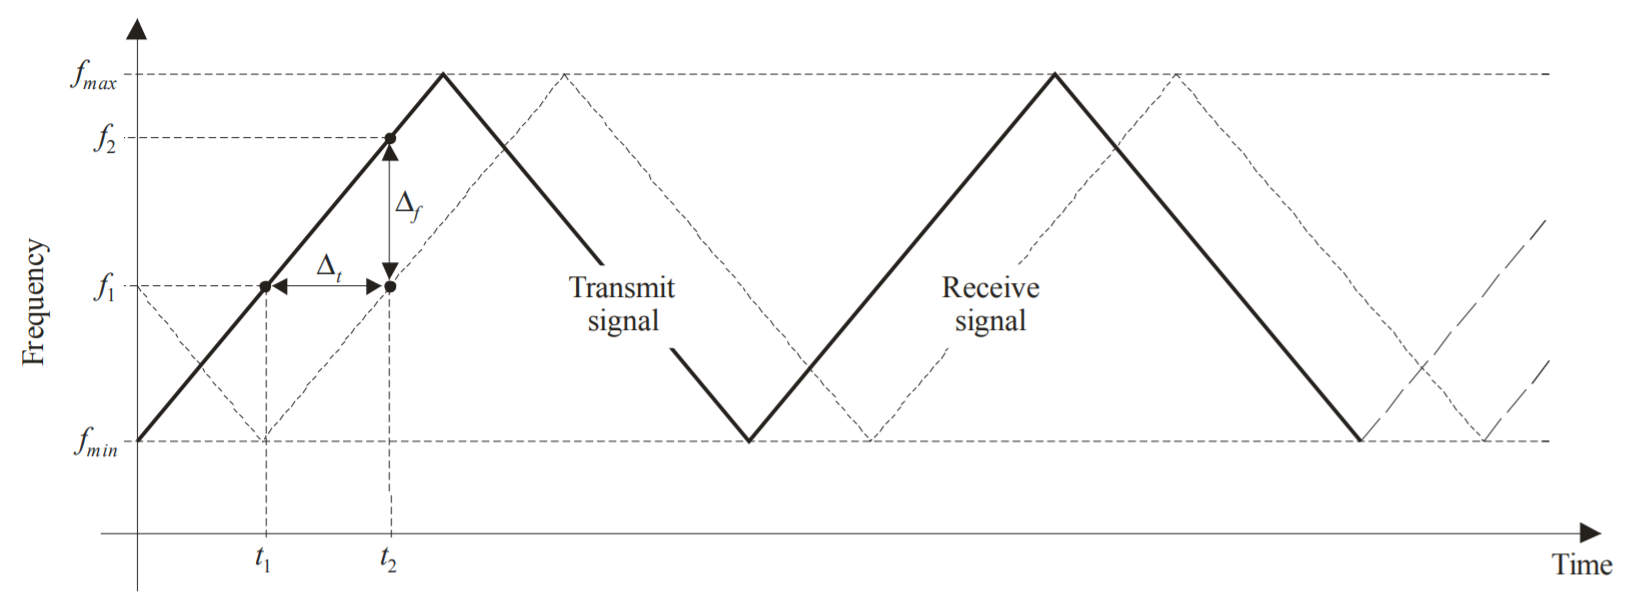
\includegraphics[scale=1.4]{FMCW_Example.PNG}
 \caption{FMCW Waveform from ITU-R M.2059-0 ~\cite{noauthor_operational_2014}}
 \label{fig:FMCW}
\end{figure}
The signal travel time is based on the return of a signal of the same frequency as the transmit signal~\cite{noauthor_operational_2014}. One method for calculating the travel time of a signal involves taking the difference between the frequency of the return signal at the current time and the frequency of the transmit signal at the current time, $\Delta f$. As shown in Figure~\ref{fig:FMCW}, given a constant waveform, the return time of a signal is:
\begin{equation*}
\Delta t = \frac{\Delta f}{df/dt} .
\end{equation*}
Once $\Delta t$ is calculated, it the height can be determined using the speed of light: 
\begin{equation*}
H = \frac{c\Delta t}{2} .
\end{equation*}
While not relying on a frequency modulated waveform, pulsed radar altimeters use a series of discrete pulses to track the current height of the aircraft. The $\Delta t$ between two pulses is used to calculate the height in the same manner that an FMCW altimeter does. 

\subsection{Altimeter Signal Processing}
The basic altimeter receiver uses a homodyne detection scheme to extract data from the received waveforms. A basic diagram of this receiver is shown in Figure~\ref{fig:homodyne}. At an instant in time, the waveform actively being transmitted is sampled and fed into the receiver mixer. All received signals are then down converted to baseband. Newer models apply digital signal processing to the downconverted signal. This is accomplished by applying an FFT to the received signal so that that all processing can be done in the frequency domain. Transformed data is passed to proprietary decision algorithms which perform an altitude estimation. Other altimeters may count the zero crossings of the received signal to determine its frequency~\cite{noauthor_operational_2014}. Some units use altitude gain control and vary sweep characteristics with altitude. Pulsed altimeters use a time gating method as opposed to the frequency domain method described here for FMCW altimeters. 

The varying methods of extracting the altitude data make the effects of interference unpredictable. Narrow band signals might cause occasional false readings, while signals spread across the band effectively raise the noise floor of the radar. Digital algorithms which rely on sufficient SNR to function may enter a fail state if the noise floor is raised too much resulting in ``Non Computed Data-points'' or NCDs~\cite{noauthor_operational_2014}.
\begin{figure}
 \centering
 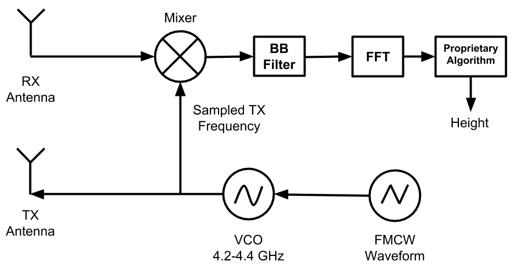
\includegraphics[scale=1.4]{homodyne_rx.png}
 \caption{Basic Diagram of Homodyne Receiver Used in Radio Altimeters}
 \label{fig:homodyne}
\end{figure}
\subsection{Radio Altimeter Antennas}
Radio altimeter antennas require a wide half power (3dB) beamwidth to allow the unit to function under all pitch and roll angles performed in flight. A 60 degree beamwidth was chosen for these tests because it is the most commonly used in industry. Typically patch antennas are used which results in a narrow bandwidth. The authors of~\cite{noauthor_operational_2014} found no specification for cross pol isolation for altimeter antennas in production, which eliminates a potential method of protecting altimeters from interferers. The authors also found that the necessary orientation of an altimeter antenna toward the ground makes it vulnerable to all possible radiation sources without shielding~\cite{noauthor_operational_2014} DO-155~\cite{noauthor_minimum_1974} specified standard antenna beamwidths for different altimeter installations. 

\subsection{Attenuation of the Altimeter Signal in Free Space}
A signal traveling from Altimeter transmit and back to receive passes through multiple different sources of gain and attenuation. There is attenuation from cable losses, gain from the TX antenna, free space path loss as the signal travels toward the ground, loss from the scattering of the signal by the ground, path loss of the return signal, a gain from the receive antenna, and finally the attenuation from return cable losses. The combination of each of these gains and losses comprises the external loop-loss $L$ for a signal leaving an aircraft. DO-155 operating standard~\cite{noauthor_minimum_1974} defines the loop loss as the ratio of the power received by the RX antenna, $P_R$ to the power sent by the transmit antenna, $P_T$:
$$ L = \frac{P_R}{P_T}.$$
The DO-155 standard specifies loop loss for different heights, standardized antennas,  ground scattering environments, and standardized cable attenuations. The standard expands the formula shown here to incorporate these effects~\cite{noauthor_minimum_1974}.

\subsection{Conclusions}
Radio Altimeters are a safety critical system in any commercial aircraft, the output of which is used by other important airborne systems. Altimeters use the time it takes a signal to travel to the ground and back to calculate the height of an aircraft off the ground, and must be able to pick up a return signal which has been attenuated significantly depending on the height. To test radio altimeters in a lab setting, both the time delay and attenuation experienced by a real signal must be simulated. 

